\documentclass{article}

\usepackage{graphicx}
\usepackage{amsfonts,amsmath,amssymb,amsthm}
\usepackage{url}
\usepackage[usenames]{color}
\usepackage[]{algorithm2e}
\usepackage{minted}
\usepackage{booktabs}

\newcommand{\figref}[1]{Figure~\ref{#1}}

\pagestyle{empty} \addtolength{\textwidth}{1.0in}
\addtolength{\textheight}{0.5in} \addtolength{\oddsidemargin}{-0.5in}
\addtolength{\evensidemargin}{-0.5in}
\newcommand{\ruleskip}{\bigskip\hrule\bigskip}
\newcommand{\nodify}[1]{{\sc #1}} \newcommand{\points}[1]{{\textbf{[#1
points]}}}

\newcommand{\bitem}{\begin{list}{$\bullet$}%
{\setlength{\itemsep}{0pt}\setlength{\topsep}{0pt}%
\setlength{\rightmargin}{0pt}}} \newcommand{\eitem}{\end{list}}

%\input{../../defs}

\newcommand{\G}{\mathcal{G}}

%\newcommand{\bE}{\mbox{\boldmath $E$}}
%\newcommand{\be}{\mbox{\boldmath $e$}}
%\newcommand{\bU}{\mbox{\boldmath $U$}}
%\newcommand{\bu}{\mbox{\boldmath $u$}}
%\newcommand{\bQ}{\mbox{\boldmath $Q$}}
%\newcommand{\bq}{\mbox{\boldmath $q$}}
%\newcommand{\bX}{\mbox{\boldmath $X$}}
%\newcommand{\bY}{\mbox{\boldmath $Y$}}
%\newcommand{\bZ}{\mbox{\boldmath $Z$}}
%\newcommand{\bx}{\mbox{\boldmath $x$}}
%\newcommand{\by}{\mbox{\boldmath $y$}}
%\newcommand{\bz}{\mbox{\boldmath $z$}}

\newcommand{\true}{\mbox{true}}
\newcommand{\Parents}{\mbox{Parents}}

\newcommand{\ww}{{\bf w}}
\newcommand{\xx}{{\bf x}}
\newcommand{\yy}{{\bf y}}
\newcommand{\real}{\ensuremath{\mathbb{R}}}


\newcommand{\eat}[1]{}

\newcommand{\CInd}[3]{({#1} \perp {#2} \mid {#3})}
\newcommand{\Ind}[2]{({#1} \perp {#2})}

\setlength{\parindent}{0pt} \setlength{\parskip}{0.5ex}
\begin{document}
\pagestyle{myheadings} \markboth{}{DS-GA-1005/CSCI-GA.2569 Problem Set
  3 -- Due Tuesday, Oct 17 }

{\LARGE
\begin{center}Inference and Representation, Fall 2017\end{center}
}

{\Large
Problem Set 4: PCA and factor analysis.
}
\begin{center}
Zhuoru Lin\\
zlin@nyu.edu
\end{center}


%{\bf Selected solutions}\\
\ruleskip 
{\em Disclaimer: 
I adhered to NYU honor code in this assignment. }
\begin{enumerate}
\item Non-Negative  matrix factorization
\begin{enumerate}
\item Likelihood
Solution:\\
Let $\lambda_{ij}=(WH)_{ij}$. For $i,j$ we have that the probability: $p(X_{ij}=x_{ij})=e^{
\lambda_{ij}} \frac{\lambda_{ij}^{x_ij}}{x_{ij}!}$. Let's write $p(X_{ij}=x_{ij})$ as $p(x_{ij})$. The log-likelihood can be calculated as:
\begin{align}
L_{ij} &= \log (p(x_{ij})) \notag \\ 
&=\lambda_{ij} + x_{ij} \log(\lambda_{ij}) - \log(x_{ij}!) \label{eqn2}
\end{align}
$log(x_{ij}!)$ in equation (\ref{eqn2}) is independent of $W$ and $H$. Therefore, we can claim that the likelihood $L(W,H)$ to be:
\begin{equation}
L(W,H) = \sum_{i,j} x_{ij} \log((WH)_{ij}) - (WH)_{ij} \label{likelihood}
\end{equation}
up to a constant.
\end{enumerate}

\pagebreak
\begin{enumerate}
\item By the definition of minorize, we must have:
\begin{align}
f(x^{t})&=g(x^{t}, x^{t}). \notag
\end{align}
Since $x^{t+1} = \arg \max_{x} g(x, x^{t})$:
\begin{equation}
g(x^t, x^t) \leq g(x^{t+1}, x^{t}). \notag
\end{equation}
Again by definition of minorize:
\begin{equation}
g(x^{t+1}, x^{t}) \leq f(x^{t+1}) \notag
\end{equation}
Combine the inequalities above, we have $F(x^{t}) \leq f(x^{t+1})$.
\pagebreak

\item \label{question_log_concave}
The concavity of logarithm directly prove the equation by:
\begin{align}
\log ( \sum_{k \leq r} y_{k} ) &= \log ( \sum_{k \leq r} c_{k} \frac{y_{k}}{c_{k}}) \notag \\
& \geq \sum_{k \leq r} c_{k} \log (\frac{y_{k}}{c_{k}}) \label{log_inequality}
\end{align}
\pagebreak

\item \label{question_inequality}
This statement follows directly by setting $c_{k}=c_{kij}$ and $y_k = w_{ik} h_{kj}$ in equation (\ref{log_inequality}) in section (\ref{question_log_concave}).
\begin{equation}
log (\sum_{k \leq r} w_{ik}h_{kj}) \geq \sum_{k \leq r} c_{kij} \log(\frac{w_{ik}h_{kj}}{c_{kij}}) \label{eqn_wh_log_inequality}
\end{equation}

\pagebreak

\item 
We first show that $g(W, H; W^{t}, H^{t}) \leq L(W, H)$:
\begin{align}
g(W, H; W^{t}, H^{t}) &= \sum_{i, j, k} [x_{ij} c_{kij}(\log(w_{ik})+\log(h_{kj})) - w_{ik}h_{kj}] \\
&= \sum_{i,j} [x_{ij} \sum_{k} c_{kij}\log(w_{ik} h_{kj})- \sum_{k} w_{ik}h_{kj}] \label{eqn_g_1}
\end{align}

Since $c_{kij} \leq 1$ we must have $\log(c_{kij}) \leq 0$. We also have $x_{ij} \geq 0$  since $X$ is non-negative. Then we can transfer equation (\ref{eqn_g_1}) into an inequality:
\begin{align}
g(W, H; W^{t}, H^{t}) &\leq \sum_{i,j} [x_{ij} \sum_{k} c_{kij}\log(w_{ik} h_{kj}/c_{kij})- \sum_{k} w_{ik}h_{kj}] \label{ineq_g_1}\\
&\leq \sum_{i,j} [x_{ij} \sum_{k} \log(\sum_{k} w_{ik} h_{kj})- \sum_{k} w_{ik}h_{kj}] \\
&=L(W,H)
\end{align}
by equation (\ref{eqn_wh_log_inequality}) in section (\ref{question_inequality}). Next we would need to show $g(W, H; W^{t}, H^{t}) = L(W^t, H^t)$ when $WH=W^{t}H^{t}$ for some $W$ and $H$. This is trivial by setting $w_{ik} h_{kj}$ to be non zero only for one $k$. 
\pagebreak

\item 
By $\frac{\partial g}{\partial w_{ik}}=0$, we get:

\begin{align}
\frac{\sum_{j}x_{ij}c_{kij}}{w_{ik}} - \sum_{j} h_{kj} &= 0\\
w_{ik} &= \frac{\sum_{j}x_{ij}c_{kij}}{\sum_{j} h_{kj} }\\
w_{ik} &= w_{ik}^t \frac{\sum_{j} h_{kj}x_{ij}/(W^{t}H^{t}_{ij})}{\sum_{j} h_{kj}}.
\end{align}

By $\frac{\partial g}{\partial h_{ik}}=0$, we get:

\begin{align}
\frac{\sum_{j}x_{ij}c_{kij}}{h_{kj}} - \sum_{j} w_{ik} &= 0\\
h_{kj} &= \frac{\sum_{i}x_{ij}c_{kij}}{\sum_{i} w_{ik} }\\
h_{kj} &= h_{kj}^t \frac{\sum_{i} w_{ik}x_{ij}/(W^{t}H^{t}_{ij})}{\sum_{i} w_{ik}}.
\end{align}
\end{enumerate}
\pagebreak

\item NMF vs PCA on images
\begin{enumerate}
\item 
\begin{figure}[ht]
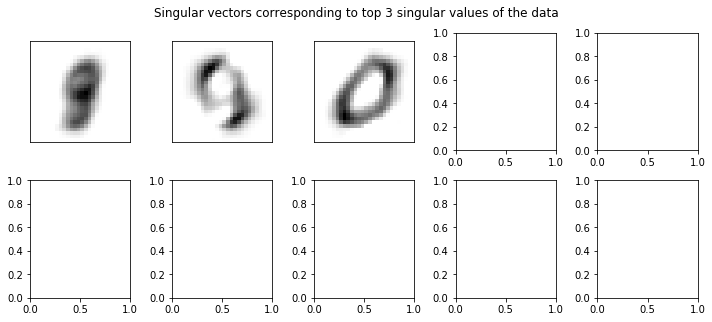
\includegraphics[width=\textwidth]{../plots/2a-1.png}
\caption{H rows when r=3}
\label{fig_r3}
\end{figure}
\begin{figure}[ht]
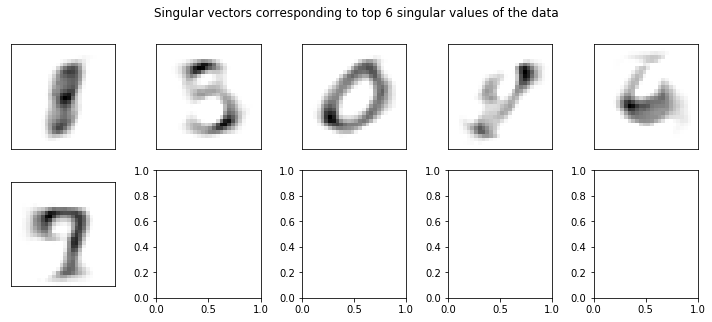
\includegraphics[width=\textwidth]{../plots/2a-2.png}
\caption{H rows when r=6}
\label{fig_r6}
\end{figure}
\begin{figure}[ht]
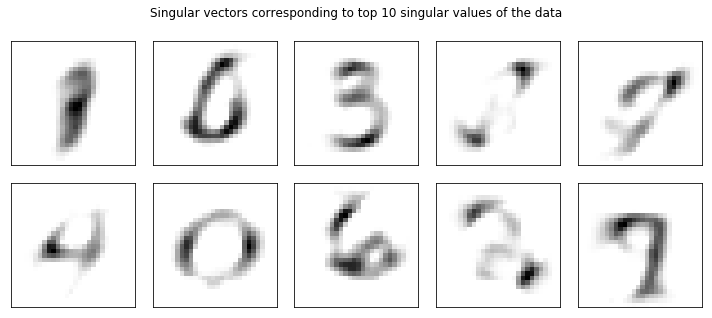
\includegraphics[width=\textwidth]{../plots/2a-3.png}
\caption{H rows when r=10}
\label{fig_r10}
\end{figure}
\pagebreak
I implemented NMF as shown below:
\begin{minted}{python}
def NMF(input_data, r=3, n_iters=10):
    X = input_data.copy()
    N, p = input_data.shape
    # Initialize W and H
    W = np.ones((N, r), dtype=np.float64)
    H = np.ones((r, p), dtype=np.float64)
    for _ in range(n_iters):
        # Update rows of W
        for k in range(r):
            H_rsum = np.sum(H[k,:])
            WH = np.dot(W,H)
            WH[np.where(WH==0)] +=0.001
            if(H_rsum!=0):
                W[:, k] = W[:, k] * np.sum(H[k,:]*(X/WH),1)/ H_rsum
        for k in range(r):
            W_rsum = np.sum(W[:,k])
            WH = np.dot(W,H)
            WH[np.where(WH==0)] +=0.001 
            if(W_rsum!=0.0):
                H[k, :] = H[k, :] * np.sum(W[:, k].reshape(N,1)*(X/WH),0)/W_rsum    
    return H
\end{minted}
The results are shown in Figure \ref{fig_r3}, \ref{fig_r6} and \ref{fig_r10}.
\pagebreak

\item Nearest neighbor search
I chose r=13 and the nearest neighbor correspond to the exact same digits as the original images. Results are shown in Figure \ref{fig_nb}.
\begin{figure}[ht]
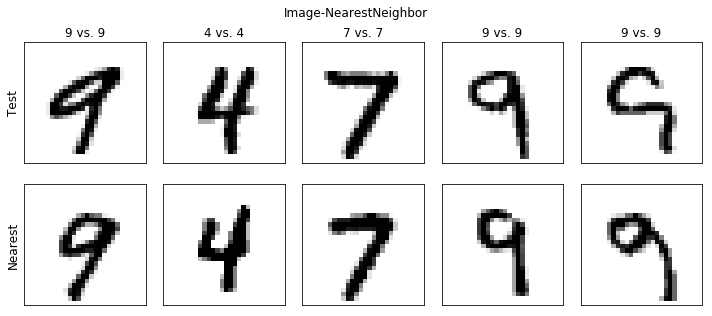
\includegraphics[width=\textwidth]{../plots/2b.png}
\caption{Nearest neighbors when r=13}
\label{fig_nb}
\end{figure}


\pagebreak
\item NMF vs PCA
Let's look at the H computed using NMF and PCA and r=10, (Figure \ref{fig_pca_nmf}). The NMF extracts digit-like components while PCA's H are more like the compose of digits.
\begin{figure}[ht]
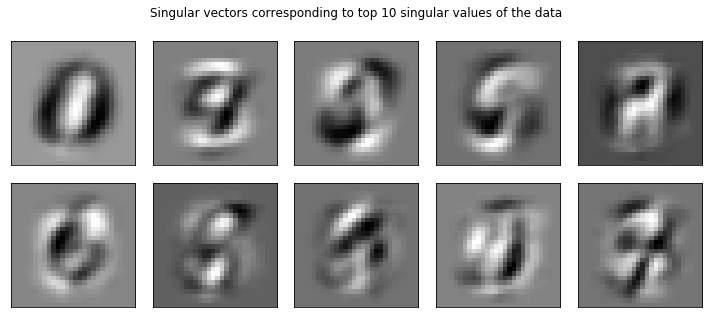
\includegraphics[width=\textwidth]{../plots/2c-pca.png}
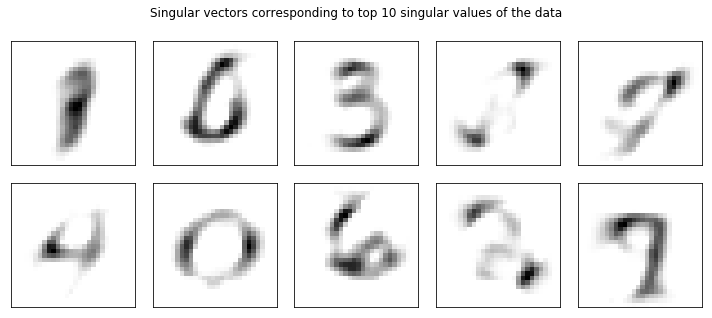
\includegraphics[width=\textwidth]{../plots/2a-3.png}
\caption{Upper: PCA, Lower: NMF}
\label{fig_pca_nmf}
\end{figure}
\end{enumerate}
\pagebreak
\item Factor Analysis, Covariance and Correlation
\begin{enumerate}
\item 
In order to show this results I need to use two lemmas:\\
\textbf{Lemma 1}: $<u, v> = E(uv)$ defines a valid inner product.
\par
\textbf{Lemma 2 (Cauchy-Schwartz inequality)}: $\lvert <u, v> \rvert^2 \leq \lvert u\rvert^2\lvert v \rvert^2$
\par
Based on these lemmas, the statement $-1 \leq \tilde{\sigma_{i,j}} \leq 1$ follows directly by setting $u=X_i-E[X_i]$ and $v=X_j - E[X_j]$.
\pagebreak
\item 
Suppose we have $X = AY + \beta$, where $X$ is observed data, $Y$ is  latent variables and $\beta$ is independent noise. By factor analysis we can decomposed the covariance matrix $\Sigma_{x} as:$
\begin{equation}
\Sigma_{x} = AA^T + B \label{eqn_factor_cov},
\end{equation}
where $B$ is the diagonal matrix formed by $B_{ii} = \beta_i$. Suppose we now apply normalization to the data $X$ and denoted the normalized $X$ as $\tilde{X}$. In this case: 
\begin{align}
\Sigma_{\tilde{X}} &= \tilde{\Sigma_{x}}\\
&= diag(\Sigma_{x})^{-\frac{1}{2}} \Sigma_{x} diag(\Sigma_{x})^{-\frac{1}{2}}\\
&=diag(\Sigma_{x})^{-\frac{1}{2}} (AA^T + B) diag(\Sigma_{x})^{-\frac{1}{2}}\\
&=\tilde{A} \tilde{A}^T + \tilde{B},
\end{align}
where $\tilde{A} = diag(\Sigma_{x})^{-\frac{1}{2}}A$ and $B=diag(\Sigma_{x})^{-\frac{1}{2}}B diag(\Sigma_{x})^{-\frac{1}{2}}$. Therefore we can still  retained the same latent variable $Y$ by making some transformation on $A$. This shows that factor analysis is robust to the change of scale. \\
However on the other hand, if we use PCA, then:
\begin{equation}
\Sigma_{x} = AA^T \label{eqn_pca_cov},
\end{equation}
At the same time we required $A$ to be orthogonal. There fore changing the scale of $X$ will result in the change of $Y$.
\pagebreak
\item 
Consider observed data $X_1, X_2, X_3$ generated by latent variable $Z_1, Z_2, Z_3$ by:
\begin{align*}
X_1 &= Z_1\\
X_2 &= X_1 + 0.001Z_2\\
X_3 &= 1000 Z_3
\end{align*}
In this example, the factor analysis will generate leading latent variable that explain the correlation between $X_1$ and $X_2$ by constructing latent variable $Z = aX_1 + bX_2$, while the PCA leading latent variable will be aligned with $X_3$ which generates most variance.
\pagebreak
\item 
Consider observed data $X_1, X_2, X_3$ generated by latent variable $Z_1, Z_2, Z_3$ by:
\begin{align*}
X_1 &= Z_1\\
X_2 &= 0.0001X_1 + 1000Z_2\\
X_3 &= 10Z_3
\end{align*}
In this case PCA should be able to catch the variable $X_2$ that contribute a lot to the covariance of the data, while Factor analysis would fail to catch $X_2$ with the weak correlation between $X_1$ and $X_2$
\pagebreak


\item 
Without proving (since we already have in DS1003), we should use the fact that if we assume $Y$ follows normal distribution $N(0, I)$ and $\epsilon$ follows normal distribution $N(0, \beta)$, then  the posterior of $X = AY + \epsilon$ must follow normal distribution $N(0, AA^T + \Sigma_{\beta})$, where $\Sigma_{\beta}$ is the covariance matrix of $\epsilon$ and $\Sigma_{\beta}=I\beta$. The posterior is proportional to the Likelihood up to a constant. That is:
 \begin{equation*}
 L(X, A, \beta) \propto N(0, AA^T + \Sigma_{\beta})
 \end{equation*}
 To optimize $A$ and $\beta$, we need to take the derivative of log likelihood with respect to $A$ and $\beta$ and set it to zero.
 \pagebreak
 
 \item 
 The parameters found by MLE is not uniquely specified. Since we should have multiple combination of $A$ correspond to the same likelihood of data. Consider a orthogonal matrix $R$, we must have: 
 \begin{equation}
 ARR^TA^T = AA^T
 \end{equation}
 Therefore we can always define $\tilde{A} = AR$ and get the exact same Likelihood:
 \begin{equation}
 L(X, \tilde{A}, \beta) = L(X, A , \beta)
 \end{equation}
 \pagebreak
 \item 
 We need to derive the solution to the maximum log-likelihood problem we mentioned before. The derivation is very long, so I borrowed the results from equation (21.2.21), Barber, D. (2012). Bayesian reasoning and machine learning. Cambridge University Press. \
 Let's suppose we are interested in finding a $H$-dimension approximation of $x$. The MLE of $A$ is given by:
 \begin{align}
 S &= \frac{1}{N}(x-\bar{x})(x-\bar{x})^T \label{eqn_sample_covariance} \\ 
 \Sigma_{\beta}^{-\frac{1}{2}} S \Sigma_{\beta}^{-\frac{1}{2}}&=U\Lambda U \label{eqn_svd}\\ 
 A &= \Sigma_{\beta}^{\frac{1}{2}}U_H(\Lambda_H-I_H)^{\frac{1}{2}} \label{eqn_MLE_A}.
 \end{align}
 The equation (\ref{eqn_sample_covariance}) is an expression of sample covariance. Equation (\ref{eqn_svd}) is a SVD of $ \Sigma_{\beta}^{-\frac{1}{2}} S \Sigma_{\beta}^{-\frac{1}{2}}$. $U$ is orthogonal eigenvectors and $\Lambda$ is the corresponding eigenvalues.  The MLE of $A$ is given by equation (\ref{eqn_MLE_A}), where $\Lambda_H$ correspond to the H largest eigenvalues and $U_H$ is a matrix formed by corresponding eigenvectors. \\
 Therefore given a known distribution of $\epsilon$ and its variance $\beta$. We can find the MLE of $A$ by going through the calculation listed above.
\end{enumerate}


\pagebreak
\item Factor Analysis vs PCA on personality data.\\
The leading factors extracted by  factor analysis and the principle components analysis  are shown in Figure \ref{fig_p4_factor} and \ref{fig_p4_pca}. This support our former conclusions that factor analysis assign leading factor to those combinations that explain most correlation. In the graph (Figure \ref{fig_p4_factor}) , those with highest  loading factor values are 'Discipline, hardwork, responsible.' which are intuitively very correlated. In PCA, these effect are not observed.

The following codes are my implementation of factor analysis:
\begin{minted}{python}
def squared_norm(x):
    return np.linalg.norm(x)**2

def svd_top_n(X,n_components):
    _, s, V = np.linalg.svd(X, full_matrices=False)
    return (s[:n_components], V[:n_components],
                        squared_norm(s[n_components:]))

def FactorAnalysis(data, n_components) :
    data = data-data.mean(0)
    n_samples, n_features = data.shape
    nsqrt = np.sqrt(n_samples)
    
    llconst = n_features * np.log(2. * np.pi) + n_components
    var = np.var(data, axis=0)
    psi = np.ones(n_features)
    loglike = []
    old_ll = -np.inf
    SMALL = 1e-12
    iteration = 10
    tol = 1e-5
    for i in range(iteration):
        sqrt_psi = np.sqrt(psi) + SMALL
        s, V, unexp_var = svd_top_n(data / (sqrt_psi * nsqrt), n_components)
        s **= 2
        
        W = np.sqrt(np.maximum(s - 1., 0.))[:, np.newaxis] * V
        del V
        W *= sqrt_psi

        # loglikelihood
        ll = llconst + np.sum(np.log(s))
        ll += unexp_var + np.sum(np.log(psi))
        ll *= -n_samples / 2.
        loglike.append(ll)
        if (ll - old_ll) < tol:
            break
        old_ll = ll

        psi = np.maximum(var - np.sum(W ** 2, axis=0), SMALL)
    return(psi,loglike[-1],W.T)
\end{minted}
\begin{figure}[ht]
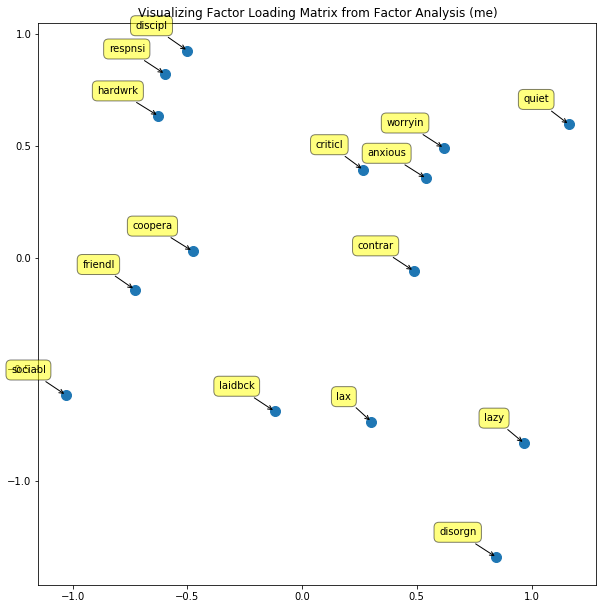
\includegraphics[width=\textwidth]{../plots/p4.png}
\caption{Factor analysis of personality data}
\label{fig_p4_factor}
\end{figure}

\begin{figure}[ht]
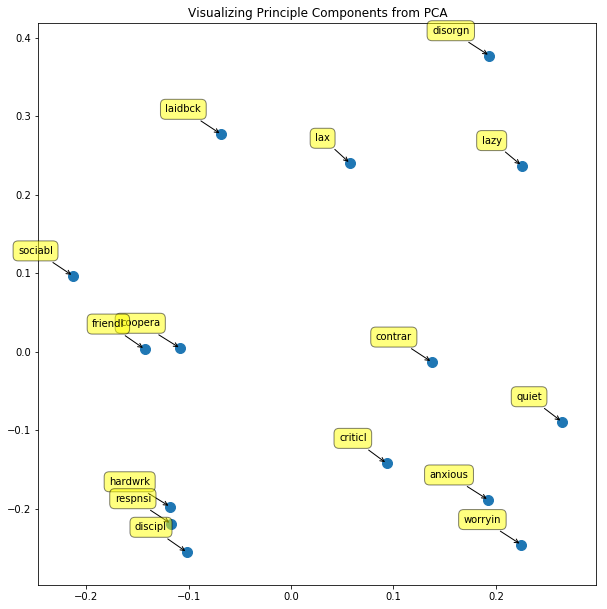
\includegraphics[width=\textwidth]{../plots/p4_pca.png}
\caption{PCA of personality data}
\label{fig_p4_pca}
\end{figure}

\end{enumerate}

\end{document}